\section{Arquitectura}
\par Tal como se ha comentado anteriormente, se procede a construir la solución de forma iterativa.
\par Debido a las funcionalidades añadidas por las últimas versiones del software, se utilizarán las últimas versiones estables de todo el software, para lo cual se descargará el código fuente y compilará según se
requiera.
\par Esto permite a su vez minimizar las dependencias entre la solución y el sistema operativo, lo que facilitará que ésta se adapte a otros sistemas si así se requiere.
\par No obstante, se utilizará como base un sistema operativo Debian GNU/Linux.

\subsection{Web Application Firewall}
\par El primer componente que se debe construir es el \acrshort{waf}. Para ello, se han definido las siguientes capas de seguridad:
\begin{enumerate}
  \item {\bf ModSecurity}. Es la primera capa de seguridad y la funcionalidad que propiamente se considera como WAF.
    \par Se utilizarán las reglas de WAF definidas por OWASP~\cite{owaspcrs}.
  \item {\bf Seguridad de la Cookie}. Se aplicarán una serie de atributos con el fin de evitar el robo o uso indebido de cookies.
  \item {\bf Cabeceras HTTP de seguridad}. Se aplicarán una serie de cabeceras HTTP que protegen contra diversos ataques.
  \item {\bf Cabecera \acrlong{hsts} (\acrshort{hsts})}. Esta cabecera HTTP evita que se realicen peticiones mediante canales no cifrados.
  \item {\bf HTTP/2}. La versión 2 de HTTP aporta una serie de mejoras respecto a las versiones anteriores en materia de seguridad y de rendimiento.
\end{enumerate}

\clearpage
\par El WAF constará pues de los componentes identificados en el {~\hyperref[fig:Diagrama_WAF_Componentes]{Diagrama del \acrshort{waf}}}
\begin{figure}[!ht]
  \centering
  \label{fig:Diagrama_WAF_Componentes}
  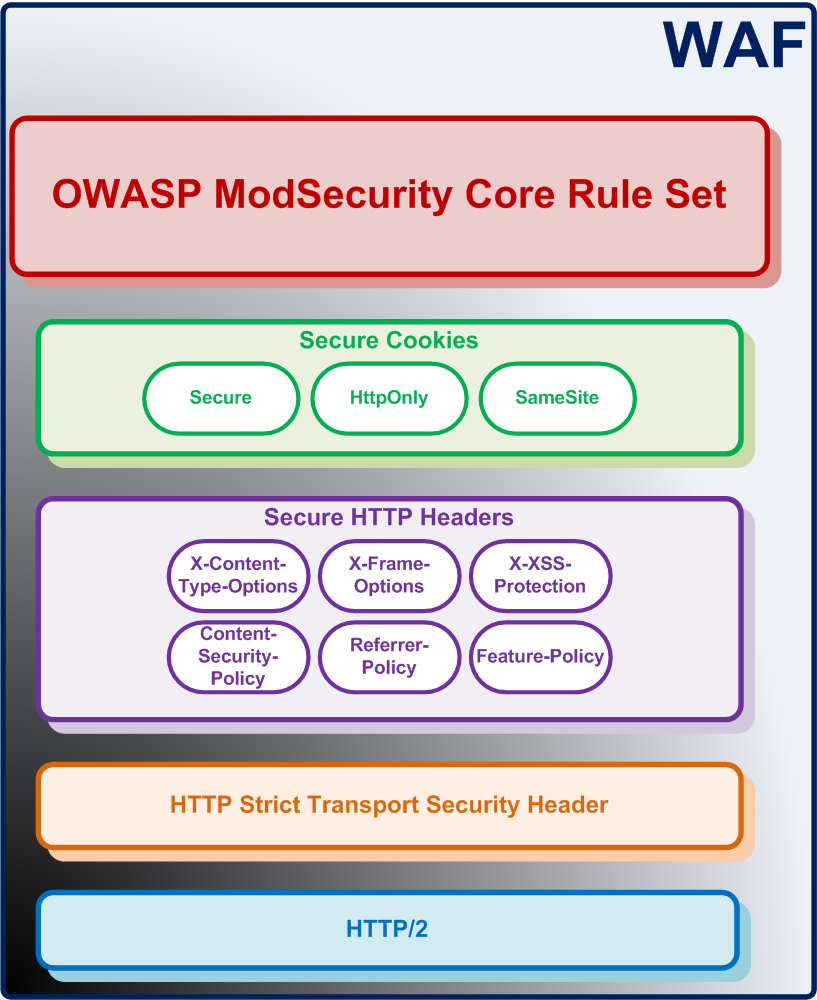
\includegraphics[width=0.7\textwidth]{fig/Diagrama_WAF_Componentes}
  \caption{Diseño de alto nivel}
\end{figure}

\subsubsection{Construcción de ModSecurity}
\par Se procede a construir el componente base sobre el que se basarán los demás componentes, esto es un WAF sobre Nginx.
\par En primer lugar se debe instalar el conector de ModSecurity.
  \lstinputlisting[language=bash,firstline=13,lastline=14]{\codePath/Docker/ccwaf/files/build/build_nginx.sh}

\par A continuación se procede a descargar e instalar la última versión disponible de Nginx. \\
\begin{minipage}{\linewidth}
  \lstinputlisting[language=bash,linerange={21-25,27-33,35-40}]{\codePath/Docker/ccwaf/files/build/build_nginx.sh}
\end{minipage}

\par Se descarga e instala ModSecurity. \\
\begin{minipage}{\linewidth}
\begin{lstlisting}[language=bash]
cd /opt/ \
git clone https://github.com/SpiderLabs/ModSecurity \
cd ModSecurity/ \
git checkout -B v3/master origin/v3/master \
sh build.sh \
git submodule init \
git submodule update \
./configure \
make \
make install \
\end{lstlisting}
\end{minipage}

\par Por último, se configura ModSecurity con una regla de bloqueo que permita realizar pruebas.\\
\begin{minipage}{\linewidth}
  \lstinputlisting[language=bash,firstline=3,lastline=33]{\codePath/Docker/ccwaf/files/build/build_modsecurity.sh}
\end{minipage}
\par El WAF envía una respuesta HTTP 403 cuando se aplica dicha regla a la petición tal como se ve en la captura ({~\hyperref[fig:WAF_test]{Respuesta de WAF a una petición no legítima}}).

\begin{figure}[!ht]
  \centering
  \label{fig:WAF_test}
  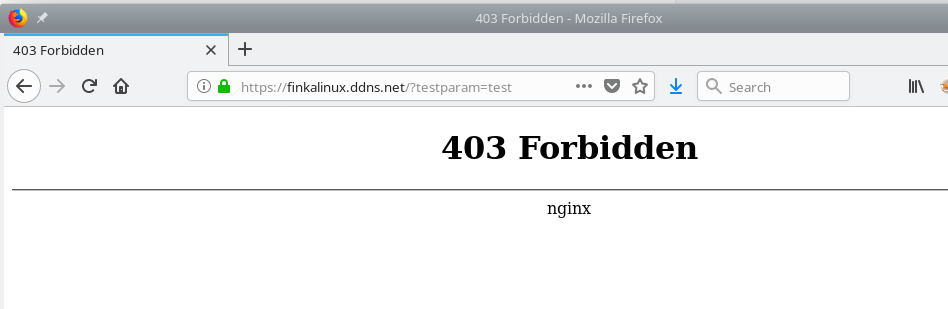
\includegraphics[width=0.7\textwidth]{fig/WAF_testparam}
  \caption{Respuesta de WAF a una petición no legítima. }
\end{figure}

\subsubsection{Soporte HTTP/2}
\par El siguiente componente que se debe añadir es el soporte en Nginx mediante el parámetro \\ \lstinline{--with-http_v2_module}.

\par Por lo que se debe compilar Nginx con los siguientes parámetros:\\
\begin{minipage}{\linewidth}
  \lstinputlisting[language=bash,linerange={24-25,27-40}]{\codePath/Docker/ccwaf/files/build/build_nginx.sh}
\end{minipage}

\par A continuación se debe  habilitar el protocolo en el fichero de configuración de nginx ({\em nginx.conf}).
\par Para ello, se modifica el parámetro {\em listen} del bloque {\em server} destinado a HTTPS:
\begin{lstlisting}[language=bash]
listen        443 ssl http2 default_server;
listen        [::]:443 ssl http2 default_server;
\end{lstlisting}

\par La segunda línea se añade con el fin de que la solución tenga soporte para IPv6.

\subsubsection{Cabecera HTTP Strict Transport Security}
\par La cabecera \acrlong{hsts}~\cite{wiki:hsts}(\acrshort{hsts} en adelante) permite implantar una política de seguridad que obliga al cliente a comunicarse mediante canales cifrados SSL/TLS.
\par Esto permite proteger el tráfico frente a ataques que puedan interceptar las comunicaciones como por ejemplo un {\em ataque de intermediario} o \gls{MitM} (en adelante \acrshort{mitm}).
\par Para habilitar esta política, se añade la siguiente cabecera a la configuración:
\begin{lstlisting}[language=bash]
add_header Strict-Transport-Security "max-age=31536000; includeSubDomains" always;
\end{lstlisting}
\par Los parámetros especificados son los siguientes:
\begin{itemize}
\item  \lstinline{max-age=31536000}. Indica la duración de la política en el cliente web. En este caso un año.
\item  \lstinline{includeSubDomains}. Indica que dicha política se debe aplicar a todos los subdominios.
\item  \lstinline{always}. Indica que la política se debe añadir a cualquier tipo de respuesta HTTP.
\end{itemize}

\subsubsection{Cabecera de seguridad {\em X-Content-Type-Options}}
\par La siguiente cabecera que se añade es {\em X-Content-Type-Options}~\cite{X-Content-Type-Options}. Esta cabecera previene que un cliente pueda realizar {\em MIME type sniffing}~\cite{mimesnif}. Esta funcionalidad representa un riesgo de seguridad debido a que permite potencialmente transformar un tipo MIME no ejecutable en ejecutable.
\par Para habilitar esta política, se añade la siguiente cabecera a la configuración:
\begin{lstlisting}[language=bash]
add_header X-Content-Type-Options "nosniff" always;
\end{lstlisting}
\par El parámetro \lstinline{nosniff} previene que el cliente aplique un tipo MIME diferente al indicado por el servidor web.
\par El parámetro \lstinline{always} tiene un comportamiento similar a lo descrito en otras cabeceras.


\subsubsection{Cabecera de seguridad {\em X-Frame-Options}}
\par Otra cabecera de seguridad a habilitar es {\em X-Frame-Options}~\cite{X-Frame-Options}. Esta cabecera previene que la petición se enmarque dentro de un frame/iframe de un dominio que no haya sido autorizado, una
técnica habitual en los ataques del tipo \gls{Clickjacking}.
\par Para habilitar esta política, se añade la siguiente cabecera a la configuración:
\begin{lstlisting}[language=bash]
add_header X-Frame-Options SAMEORIGIN always;
\end{lstlisting}
\par El parámetro \lstinline{SAMEORIGIN} indica que las peticiones sólo podrán realizarse en frames/iframes pertenecientes al mismo dominio.


\subsubsection{Cabecera de seguridad {\em X-XSS-Protection}}
\par La siguiente cabecera que se habilita es {\em X-XSS-Protection}~\cite{X-XSS-Protection}. Esta cabecera indica al navegador web que habilite y aplique el filtro contra vulnerabilidades del tipo \gls{XSS}.
\par Para habilitar esta política, se añade la siguiente cabecera a la configuración:
\begin{lstlisting}[language=bash]
add_header X-XSS-Protection "1; mode=block" always;
\end{lstlisting}
\par El parámetro \lstinline{1; mode=block} indica que el filtro contra vulnerabilidades XSS debe estar activado obligatoriamente.


\subsubsection{Cabecera de seguridad {\em Referrer-Policy}}
\par La cabecera {\em Referrer-Policy}~\cite{ReferrerPolicy} tiene como función limitar qué información se envía en la cabecera {\em Referrer}.
\par Esta cabecera se envía cuando el usuario hace click en un enlace y, por defecto, se envía la URL completa de la página actual a la nueva página. Esto implica que, si existe algún tipo de información en la URL actual, la
página web destino tendrá acceso a ella.
\par Este comportamiento puede aprovecharse para realizar ataques de falsificación de petición en sitios cruzados (en adelante \acrshort{xsrf}, del inglés \gls{xsrf}) o \gls{Phishing} entre otros.
\par Para habilitar esta política, se añade la siguiente cabecera a la configuración:
\begin{lstlisting}[language=bash]
add_header Referrer-Policy "strict-origin-when-cross-origin";
\end{lstlisting}
\par El parámetro \lstinline{strict-origin-when-cross-origin} indica lo siguiente:
\begin{itemize}
  \item Si la dirección destino es más insegura que la dirección actual (HTTPS $\rightarrow$ HTTP), no se envía ningún dato en la cabecera {\em Referrer}.
  \item Si la dirección destino pertenece al mismo dominio, se envía la URL completa.
  \item Si la dirección destino pertenece a un dominio diferente, se enviará el dominio de la dirección actual y se eliminará cualquier parámetro o ruta de la URL.
\end{itemize}

\subsubsection{Cabecera {\em Feature-Policy}}
\par La cabecera {\em Feature-Policy}~\cite{FeaturePolicy} define las funcionalidades permitidas. Se trata de una política bastante reciente cuyo borrador ha sido publicado por el \acrshort{w3c} (\acrlong{w3c}) en abril de 2019~\cite{FeaturePolicyDraft}.
\par Actualmente se han publicado las siguientes directivas:
\begin{multicols}{2}
\begin{itemize}
	\item ambient-light-sensor
	\item autoplay
	\item accelerometer
	\item camera
	\item display-capture
	\item document-domain
	\item encrypted-media
	\item execution-while-not-rendered
	\item execution-while-out-of-viewport
	\item fullscreen
	\item geolocation
	\item loading-frame-default-eager
	\item loading-image-default-eager
	\item gyroscope
	\item magnetometer
	\item microphone
	\item midi
	\item payment
	\item picture-in-picture
	\item speaker
	\item sync-xhr
	\item usb
	\item wake-lock
	\item vr / xr
\end{itemize}
\end{multicols}

\par Se han definido las siguientes políticas con el fin de garantizar compatibilidad sin sacrificar la seguridad. \\
\begin{minipage}{\linewidth}
  \lstinputlisting[language=bash,firstline=103,lastline=116]{\codePath/Docker/ccwaf/files/nginx_conf/snippets/security_headers.conf}
\end{minipage}

\par Los valores elegidos son:
\begin{itemize}
  \item \lstinline{'self'}. Indica que la funcionalidad está permitida en las peticiones al dominio y en peticiones dentro de los iframes que pertenezcan al mismo dominio.
  \item \lstinline{'none'}. Indica que la funcionalidad no está permitida.
\end{itemize}

\par Se espera ir ajustando los parámetros a medida que se implementen estas políticas en distintos entornos y evolucionen las directivas.


\subsubsection{Cabecera de Políticas de Seguridad de Contenido}
\par La cabecera de Políticas de Seguridad de Contenido~\cite{csp} (en adelante \acrshort{csp}, del inglés \acrlong{csp}) define una serie de directivas de seguridad que permiten proteger la plataforma
de ataques \gls{XSS} o \gls{SQLI}.
\par Estas políticas son muy versátiles pero también pueden provocar que el contenido no se entregue adecuadamente.
\par Para prevenirlo, se ha identificado el contenido multimedia y las redes sociales más comunes:
\begin{multicols}{2}
\begin{itemize}
  \item 500px.com
  \item 500px.org
  \item cloudflare.com
  \item facebook.com
  \item facebook.net
  \item flickr.com
  \item google-analytics.com
  \item googleapis.com
  \item google.com
  \item imgur.com
  \item jquery.com
  \item reddit.com
  \item staticflickr.com
  \item youtube.com
\end{itemize}
\end{multicols}

\par Utilizando estos servicios como referencia, se han codificado las siguientes listas: \\
\begin{minipage}{\linewidth}
  \lstinputlisting[language=bash,linerange={40-70}]{\codePath/Docker/ccwaf/files/nginx_conf/snippets/security_headers.conf}
\end{minipage}

\par Por último, se ha configurado y habilitado la cabecera \acrshort{csp} como se muestra a continuación: \\
\begin{minipage}{\linewidth}
  \lstinputlisting[language=bash,linerange={77-82,85-88}]{\codePath/Docker/ccwaf/files/nginx_conf/snippets/security_headers.conf}
\end{minipage}

\subsubsection{Control de seguridad de {\em Cookies}}
\par Otro elemento que se deben proteger son las cookies de la plataforma web (\gls{Cookie}), para ello el WAF modificará las cookies de la plataforma web añadiendo los siguientes atributos si no estuviesen previamente:
\begin{itemize}
  \item Secure. Previene que la cookie sea enviada mediante canales no cifrados.
  \item HttpOnly. Previene que la cookie sea accesible por un medio que no sea HTTP/HTTPS. Por lo tanto la cookie no puede ser accesible por un script en el navegador, lo que proporciona protección contra ataques de
    \acrshort{xss}.
  \item SameSite. Previene que la cookie se envíe a un dominio diferente, por lo que ayuda a proteger la plataforma frente a ataques \gls{XSRF}.
    \par Debido a que es una práctica habitual el uso de la misma cookie en distintos dominios se ha optado por aplicar este filtro en una modalidad más permisiva: \lstinline{SameSite=Lax}. Esta opción evita que se envíe
    la cookie en peticiones POST entre otras.
\end{itemize}

\par Nginx por defecto soporta esta funcionalidad para la pagina raíz ("{\em /}"), pero esta protección no se aplica a las demás páginas.
\par Para solucionarlo se hace uso de un módulo externo, \lstinline{nginx_cookie_flag_module}~\cite{nginx_cookie}, con este módulo se pueden habilitar los atributos identificados a todas las cookies con independencia de la URL.
\par En primer lugar se debe descargar el módulo.
  \lstinputlisting[language=bash,firstline=17,lastline=18]{\codePath/Docker/ccwaf/files/build/build_nginx.sh}

\par A continuación se debe modificar la compilación de Nginx añadiendo el siguiente parámetro \\ \lstinline{--add-module=../nginx_cookie_flag_module}.

\par Y se compila Nginx con los siguientes parámetros:\\
\begin{minipage}{\linewidth}
  \lstinputlisting[language=bash,linerange={24-38}]{\codePath/Docker/ccwaf/files/build/build_nginx.sh}
\end{minipage}

\subsection{Software criptográfico}
\par Se procede a configurar las comunicaciones HTTPS.
\par Para ello, lo primero será crear un certificado auto-firmado de pruebas con su correspondiente clave privada. \\
\begin{minipage}{\linewidth}
  \lstinputlisting[language=bash,linerange={3-10,62-64}]{\codePath/Docker/ccwaf/files/build/build_nginx.sh}
\end{minipage}

\par A continuación se debe configurar Nginx para que ofrezca este certificado a los clientes.\\
\begin{minipage}{\linewidth}
  \lstinputlisting[language=bash,linerange={29-31,47-55}]{\codePath/Docker/ccwaf/files/nginx_conf/sites-available/default.conf.template}
\end{minipage}
\par Siendo:
\begin{itemize}
  \item \lstinline{listen}. Indica el puerto donde el servicio está escuchando sobre IPv4 e IPv6, usando canales cifrados SSL, HTTP/2 y siendo el servicio por defecto.
  \item \lstinline{ssl_certificate}. Indica la clave privada y el certificado que se han creado anteriormente.
  \item \lstinline{ssl_session_cache}. Indica cómo gestionar la caché de las sesiones SSL.
  \item \lstinline{ssl_session_timeout}. Indica el tiempo de vida de la sesión SSL en caso de inactividad. Dado que la negociación SSL tiene un coste computacional elevado, es preferible mantener las sesiones inactivas en
    caso de que se vayan a retomar.
  \item \lstinline{ssl_protocols}. Indica las versiones de TLS compatibles. Por defecto se utiliza la versión superior que soporte el cliente.
  \item \lstinline{ssl_ciphers}. Indica los algoritmos de cifrados soportados. Se desactivan algoritmos con cifrado NULL y MD5 explícitamente y sólo se permiten algoritmos considerados con seguridad criptográfica alta.
  \item \lstinline{ssl_prefer_server_ciphers}. Indica que el WAF será el responsable de elegir el algoritmo de cifrado utilizado.
\end{itemize}


\subsection{Contenedores de software}
\par Se ha elegido Docker como tecnología de contenedores.
\par Para construir y probar la solución se han definido los siguientes contenedores:
\begin{itemize}
  \item {\em ccwaf}. Contenedor sobre el que se despliegan los componentes WAF vistos.
  \item {\em letsencrypt}. Contenedor sobre el que se configurará el gestor de certificados que aprovisionará a los demás servicios web con certificados creador por una entidad certificadora de confianza.
  \item {\em basicwebserver}. Contenedor en el que se desplegará un servicio web básico. Este elemento se podrá eliminar una vez la solución esté funcionando en el entorno de producción, pero se distribuirá como parte de
    la solución para facilitar las tareas de configuración y depuración de errores.
\end{itemize}
\par Todos los contenedores se han construido sobre una imagen base de Debian GNU/Linux del repositorio de Docker Hub ({\em debian:buster-slim}~\cite{dockerhubdebian}).
\par Se puede consultar el código en el apéndice (~\hyperref[listing:ccwafDockerfile]{fichero Dockerfile del WAF}).

\begin{figure}[!ht]
  \centering
  \label{fig:Diagrama Docker WAF}
  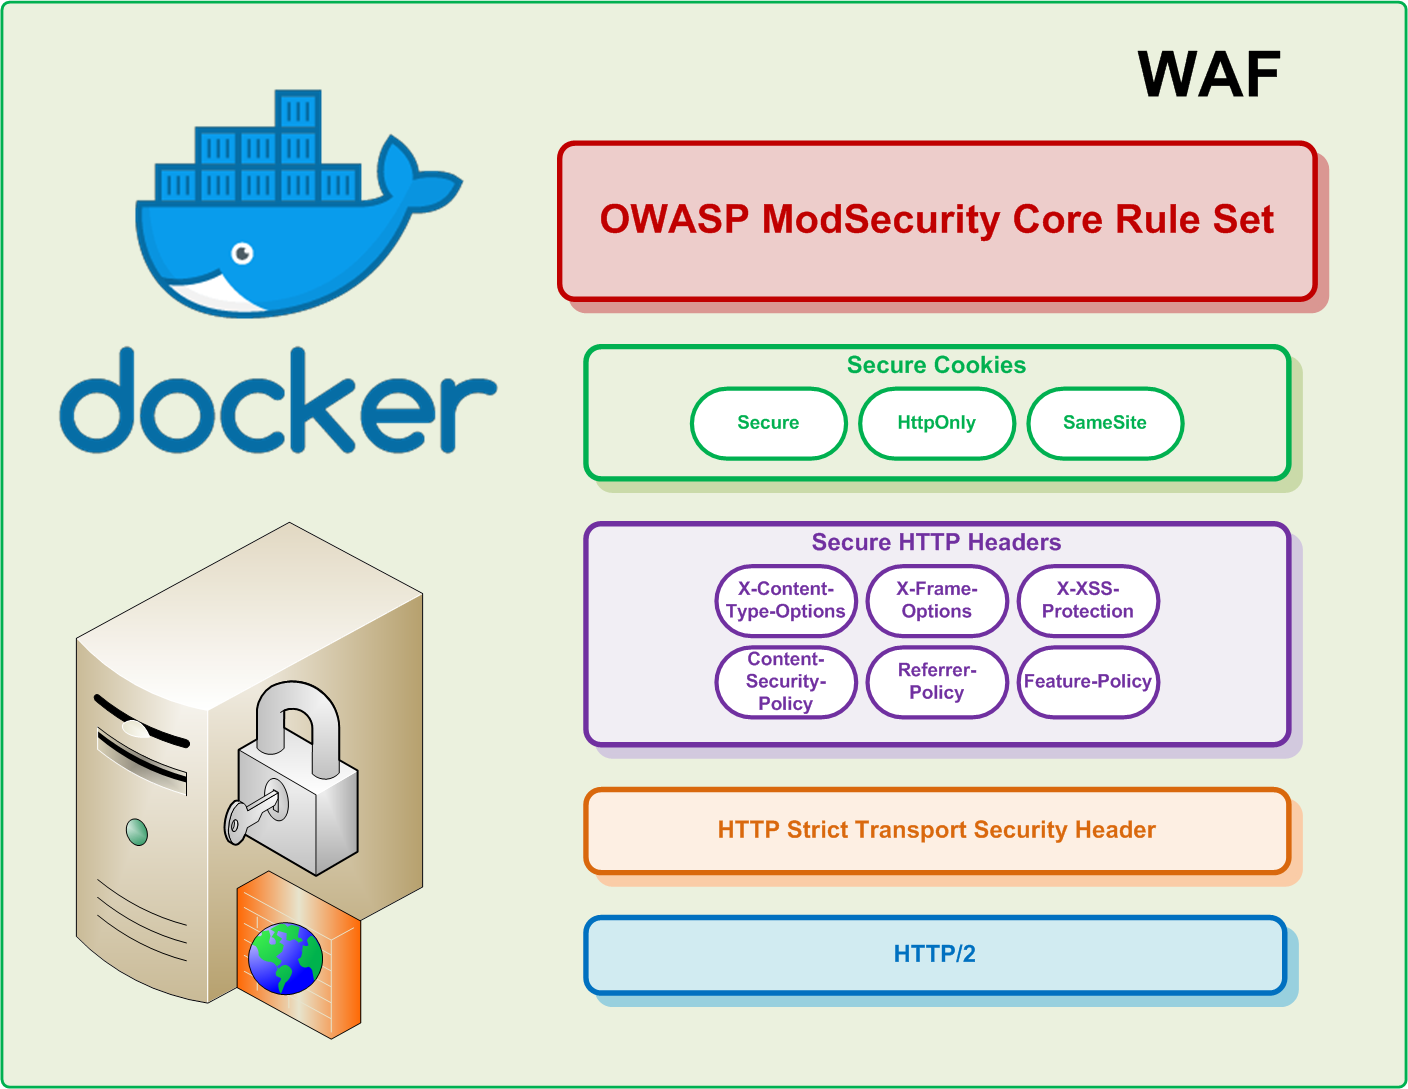
\includegraphics[width=0.7\textwidth]{fig/Diagram_Docker_WAF}
  \caption{Controles de seguridad desplegados en el contenedor Docker.}
\end{figure}

\subsection{Software de gestión de certificados HTTPS}
\par Se ha elegido Let's Encrypt para gestionar los certificados, pues permite que la gestión sea automática y no tiene coste económico.
\par En el \hyperref[fig:Diagram_LetsEncypt_LLD]{diagrama de Let's Encrypt} se puede ver cómo se han definido las comunicaciones entre la instancia de Let's Encrypt desplegada en el cluster de Kubernetes y el servicio SaaS
ofrecido por el proveedor.
\begin{figure}[!ht]
  \centering
  \label{fig:Diagram_LetsEncypt_LLD}
  \includegraphics[width=0.7\textwidth]{fig/Diagram_LetsEncypt_LLD}
  \caption{Diagrama de comunicaciones de Let's Encrypt.}
\end{figure}
\par El modo de funcionamiento es el siguiente:
\begin{enumerate}
  \item La instancia de Docker crea una clave privada.
  \item La instancia de Docker realiza una petición de certificado al servicio SaaS.
  \item El servicio SaaS le comunica una variable temporal no predecible (tipo NONCE) al cliente Let's Encrypt.
  \item La instancia de Docker crea un fichero accesible por el servicio SaaS mediante petición HTTP con el valor propuesto como nombre de fichero.
  \item La instancia de Docker responde al servicio SaaS con el fichero temporal firmado con su clave privada.
  \item El servicio SaaS realiza una petición HTTP para comprobar que la instancia de Docker tiene control sobre el dominio sobre el que se pide el certificado.
    \par La taxonomía de la petición es \lstinline{http://<dominio>:80/.well-known/acme-challenge/<variable-NONCE>}.
  \item El servicio SaaS valida la respuesta HTTP y, a continuación, valida al agente Let's Encrypt.
\end{enumerate}
\par Una vez el agente ha sido autorizado, éste podrá pedir un nuevo certificado, renovarlo o revocarlo.

\subsection{Software de automatización u orquestación}
\par Se ha elegido Kubernetes para gestionar y automatizar la solución.
\par Para ello, se han definido los siguientes elementos:
\begin{itemize}
  \item Para el WAF:
    \begin{itemize}
      \item {\em ccwaf deployment}. Es el componente encargado de desplegar las instancias de WAF.
      \item {\em ccwaf service}. Es el componente encargado de publicar los PODs desplegados y ofrecer abstracción a los servicios externos.
    \end{itemize}
  \item Para el servidor web:
    \begin{itemize}
      \item {\em basicwebserver deployment}. Es el componente encargado de desplegar las instancias de servicio web.
      \item {\em basicwebserver service}. Es el componente encargado de publicar los PODs desplegados.
    \end{itemize}
  \item Para el servidor de Let's Encrypt:
    \begin{itemize}
      \item {\em basicwebserver deployment}. Es el componente encargado de desplegar la instancia de Let's Encrypt.
      \item {\em letsencrypt service}. Es el componente encargado de publicar los PODs desplegados.
    \end{itemize}
\end{itemize}

\par A continuación se muestran los aspectos más representativos de estos elementos:

\subsubsection{ccwaf deployment}
\begin{minipage}{0.8\linewidth}
  \lstinputlisting[language=bash,caption=\lstname,linerange={27-64}]{\codePath/Kubernetes/kub_waf-server.yaml.template}
\end{minipage}
\par Se destacan los siguientes elementos:
\par \lstinline{replicas: 2}. Indica el número de instancias que se despliegan. En las pruebas se han desplegado entre dos y cinco instancias con el fin de validar múltiples instancias en la plataforma.
\par \lstinline{image: <SET_REGISTRY>/<SET_OWNER>/ccwaf:<SET_RELEASE>}. Indica el repositorio desde el que
se descargarán las imágenes. En la elaboración del proyecto se ha utilizado un repositorio propio, pero se
compartirá a un repositorio público tras realizar la entrega.
\par \lstinline{volumeMounts}. Indica el servicio de ficheros que se utilizará para compartir certificados.
Este recurso debe ser inmutable y tolerante a reconstrucciones del entorno, por lo que se ha utilizado un
servicio NFS externo a la plataforma de Kubernetes.

\subsubsection{ccwaf service}
\begin{minipage}{0.8\linewidth}
  \lstinputlisting[language=bash,caption=\lstname,linerange={1-23}]{\codePath/Kubernetes/kub_waf-server.yaml.template}
\end{minipage}
\par En esta configuración destaca el parámetro \lstinline{type: NodePort}, pues el valor {\em NodePort}
indica que el WAF será accesible externamente desde Internet.

\subsubsection{ basicwebserver deployment}
\begin{minipage}{0.8\linewidth}
  \lstinputlisting[language=bash,caption=\lstname,linerange={24-61}]{\codePath/Kubernetes/kub_basicwebserver-server.yaml.template}
\end{minipage}
\par Se puede ver que este elemento es similar al desplegado para el WAF. En esta ocasión se han
desplegado entre dos y cinco instancias en las pruebas con el fin de validar que el entorno distribuido
funciona correctamente.


\subsubsection{ basicwebserver service}
\begin{minipage}{0.8\linewidth}
  \lstinputlisting[language=bash,caption=\lstname,linerange={1-20}]{\codePath/Kubernetes/kub_basicwebserver-server.yaml.template}
\end{minipage}
\par Se puede comprobar como en este servicio se ha configurado el siguiente parámetro: \lstinline{type: ClusterIP}.
\par Al utilizar el valor {\em ClusterIP} se define que las instancias gestionadas por este servicio sólo
son accesibles internamentes al cluster de Kunernetes y, por lo tanto, no son accesibles desde Internet.
\par Con esto se garantiza que las peticiones que se realicen a la plataforma web deben provenir
forzosamente del WAF, con lo que {\bf se garantiza que los mecanismos de protección del WAF serán
aplicados}.

\subsubsection{ basicwebserver deployment}
\begin{minipage}{0.8\linewidth}
  \lstinputlisting[language=bash,caption=\lstname,linerange={24-61}]{\codePath/Kubernetes/kub_basicwebserver-server.yaml.template}
\end{minipage}
\par En esta ocasión se ha desplegado una única réplica, pues este servicio está dedicado a la gestión de
certificados, un servicio al que los usuarios no tienen acceso y con un consumo menor de recursos.

\subsubsection{ letsencrypt service}
\begin{minipage}{0.8\linewidth}
  \lstinputlisting[language=bash,caption=\lstname,linerange={1-20}]{\codePath/Kubernetes/kub_basicwebserver-server.yaml.template}
\end{minipage}
\par Al igual que en el servicio web, se ha optado por proteger el servicio Let's Encrypt con el WAF, por
lo que se ha definido nuevamente \lstinline{type: ClusterIP}.


\subsection{Diseño final}
\par Tras construir todos los componentes necesarios, las peticiones HTTP y HTTPS son tal como se indica en el \hyperref[fig:Diagram_HTTP_Services]{Diagrama de peticiones HTTP/HTTPS en la solución}.
\begin{figure}[!ht]
  \centering
  \label{fig:Diagram_HTTP_Services}
  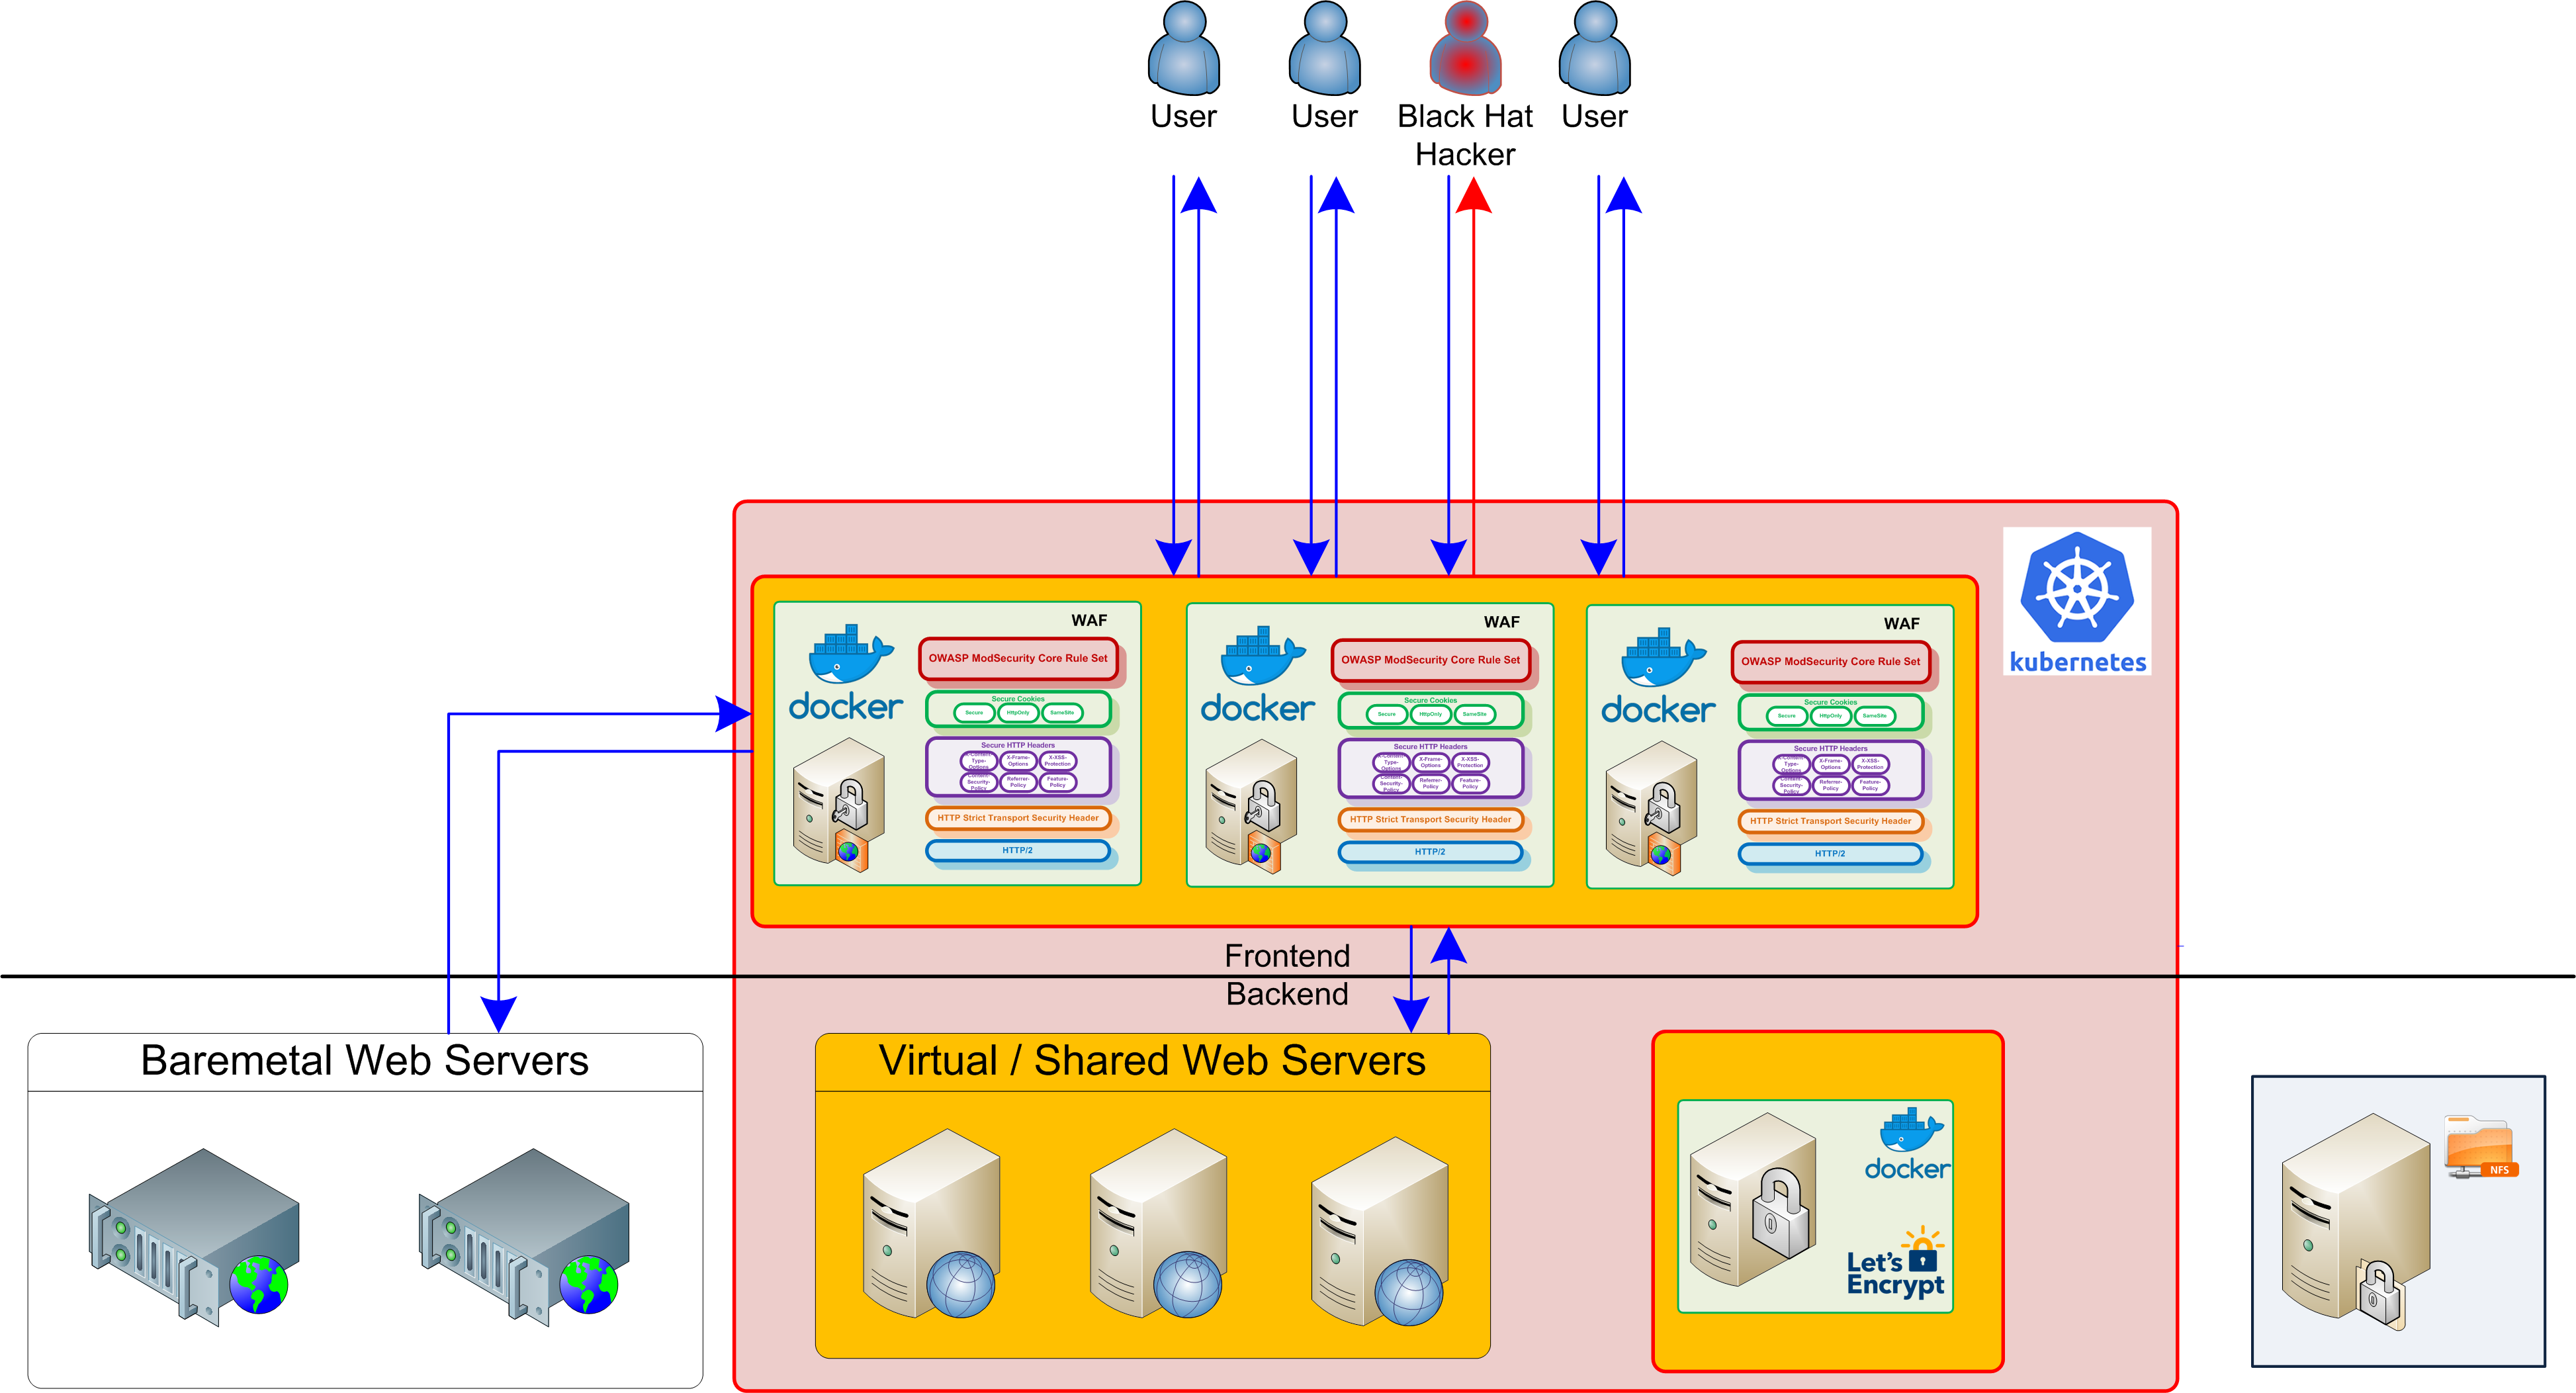
\includegraphics[width=\textwidth]{fig/Diagram_HTTP_Services}
  \caption{Diagrama de peticiones HTTP y HTTPS}
\end{figure}
